\documentclass{article}
\usepackage[utf8]{inputenc}
\usepackage{amsmath}
\usepackage{graphicx}
\usepackage{hyperref}
\usepackage{listings}
\usepackage{biblatex} 
\addbibresource{biblio.bib}
\usepackage{graphicx}

\title{Sciences humaines, sciences sociales à l'ère numérique : la mise en données et méthodes de modélisation des connaissances}
\author{
    Stéphane Pouyllau\\
    \textit{Ingénieur de recherche hors classe CNRS} \\
    \textit{Professeur attaché à l'université d'Evry-Paris-Saclay}\\
    \textit{Orcid : 0000-0002-9619-1002}
}
\date{Séance du 18 novembre 2024}


\begin{document}

\maketitle

\section{Introduction (10 minutes)}
\subsection{Présentation du cours}
\begin{itemize}
    \item Objectifs du cours
    \item Importance de la structuration des données\cite{hooland2016}
    \item Aperçu des formats CSV, SGBDR, XML (TEI), et RDF  
\end{itemize}

\begin{figure}
    \centering
    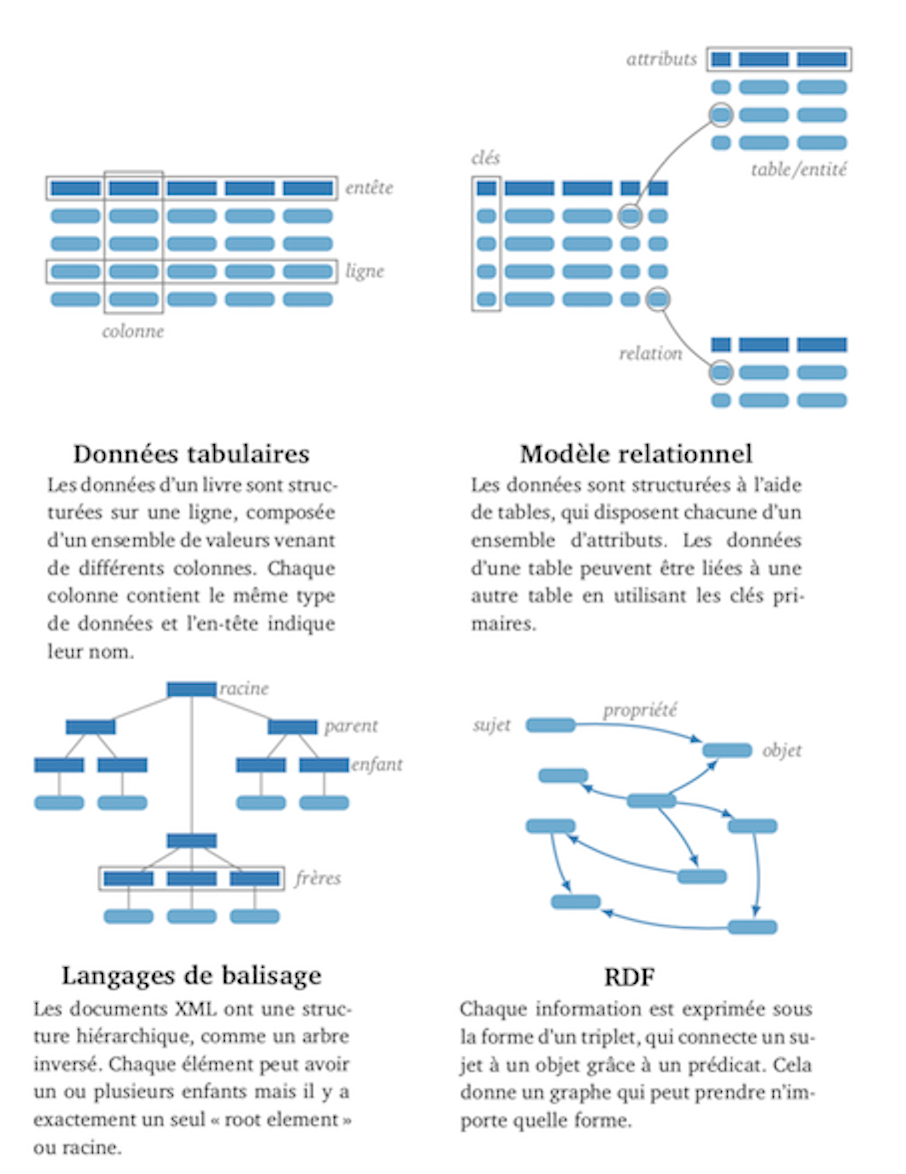
\includegraphics[width=0.5\linewidth]{fig/Setl.png}
    \caption{Seth van Hooland \& al., 2016.}
    \label{fig:enter-label}
\end{figure}

\subsection{Contexte et applications}
\begin{itemize}
    \item Utilisations courantes de chaque format
    \item Exemples d'industries et de cas d'utilisation
\end{itemize}

\section{Partie 1 : CSV (20 minutes)}
\subsection{Introduction à CSV}
\begin{itemize}
    \item Définition et historique
    \item Structure de base d'un fichier CSV
\end{itemize}

\subsection{Syntaxe CSV}
\begin{itemize}
    \item Séparateurs de colonnes et de lignes
    \item Gestion des valeurs manquantes
    \item Exemple de fichier CSV
\end{itemize}

\begin{lstlisting}[language=CSV, caption=Exemple de fichier CSV]
name,age,city
Alice,30,New York
Bob,25,Los Angeles
Charlie,35,Chicago
\end{lstlisting}

\subsection{Avantages et inconvénients}
\begin{itemize}
    \item Simplicité et lisibilité
    \item Limitations en termes de structure et de types de données
\end{itemize}

\subsection{Exercice pratique}
\begin{itemize}
    \item Créer un fichier CSV
    \item Importer et manipuler des données CSV avec un outil de tableur (Excel, Google Sheets)
\end{itemize}

\section{Partie 2 : Modèle Relationnel (SGBDR) (20 minutes)}
\subsection{Introduction au modèle relationnel}
\begin{itemize}
    \item Définition et historique
    \item Concepts de base : tables, colonnes, lignes, clés primaires et étrangères
\end{itemize}

\subsection{Syntaxe SQL}
\begin{itemize}
    \item Création de tables
    \item Insertion de données
    \item Requêtes de sélection
    \item Exemple de schéma relationnel
\end{itemize}

\begin{lstlisting}[language=SQL, caption=Exemple de schéma relationnel en SQL]
CREATE TABLE Employees (
    EmployeeID INT PRIMARY KEY,
    FirstName VARCHAR(50),
    LastName VARCHAR(50),
    DepartmentID INT,
    FOREIGN KEY (DepartmentID) REFERENCES Departments(DepartmentID)
);

CREATE TABLE Departments (
    DepartmentID INT PRIMARY KEY,
    DepartmentName VARCHAR(50)
);
\end{lstlisting}

\subsection{Avantages et inconvénients}
\begin{itemize}
    \item Intégrité des données et transactions
    \item Complexité de gestion des relations
\end{itemize}

\subsection{Exercice pratique}
\begin{itemize}
    \item Créer un petit schéma relationnel
    \item Exécuter des requêtes SQL pour manipuler les données
\end{itemize}

\section{Partie 3 : XML (TEI) (20 minutes)}
\subsection{Introduction à XML}
\begin{itemize}
    \item Définition et historique
    \item Structure de base d'un document XML
\end{itemize}

\subsection{Syntaxe XML (TEI)}
\begin{itemize}
    \item Éléments et attributs
    \item Balises et nœuds
    \item Exemple de document XML TEI
\end{itemize}

\begin{lstlisting}[language=XML, caption=Exemple de document XML TEI]
<TEI xmlns="http://www.tei-c.org/ns/1.0">
    <teiHeader>
        <fileDesc>
            <titleStmt>
                <title>Example Document</title>
                <author>John Doe</author>
            </titleStmt>
            <publicationStmt>
                <publisher>Example Publisher</publisher>
                <date>2023</date>
            </publicationStmt>
        </fileDesc>
    </teiHeader>
    <text>
        <body>
            <p>This is an example of a TEI XML document.</p>
        </body>
    </text>
</TEI>
\end{lstlisting}

\subsection{Avantages et inconvénients}
\begin{itemize}
    \item Flexibilité et extensibilité
    \item Complexité et verbosité
\end{itemize}

\subsection{Exercice pratique}
\begin{itemize}
    \item Créer un petit document XML TEI
    \item Valider le document XML avec un outil en ligne
\end{itemize}

\section{Partie 4 : RDF (20 minutes)}
\subsection{Introduction à RDF}
\begin{itemize}
    \item Définition et historique
    \item Concepts de base : triples, sujets, prédicats, objets
\end{itemize}

\subsection{Syntaxe RDF}
\begin{itemize}
    \item Représentation en XML, Turtle, JSON-LD
    \item Exemple de document RDF
\end{itemize}

\begin{lstlisting}[language=Turtle, caption=Exemple de document RDF en Turtle]
@prefix ex: <http://example.org/> .

ex:Alice ex:knows ex:Bob .
ex:Bob ex:age 25 .
ex:Bob ex:livesIn ex:LosAngeles .
\end{lstlisting}

\subsection{Avantages et inconvénients}
\begin{itemize}
    \item Flexibilité et interopérabilité
    \item Complexité de gestion des données
\end{itemize}

\subsection{Exercice pratique}
\begin{itemize}
    \item Créer un petit document RDF
    \item Valider le document RDF avec un outil en ligne
\end{itemize}

\section{Conclusion et Q\&A (10 minutes)}
\subsection{Résumé des points clés}
\begin{itemize}
    \item Récapitulatif des formats CSV, SGBDR, XML (TEI), et RDF
    \item Comparaison des avantages et inconvénients
\end{itemize}

\subsection{Questions et réponses}
\begin{itemize}
    \item Répondre aux questions des participants
    \item Discussion ouverte sur les applications pratiques
\end{itemize}

\section{Ressources supplémentaires}
\begin{itemize}
    \item Liens vers des outils en ligne pour valider XML, manipuler CSV et visualiser des graphes.
    \item Lectures recommandées pour approfondir chaque sujet.
\end{itemize}

\section{Matériel nécessaire}
\begin{itemize}
    \item Ordinateur avec accès à Internet pour les exercices pratiques.
    \item Outils de tableur (Excel, Google Sheets) pour manipuler les fichiers CSV.
    \item Outils de gestion de bases de données relationnelles (MySQL, PostgreSQL) pour les exercices sur le modèle relationnel.
    \item Outils de validation XML pour les exercices sur XML (TEI).
    \item Outils de validation RDF pour les exercices sur RDF.
\end{itemize}

\section{Bibliographie}
\printbibliography

\end{document}